\chapter{Literature Review}
\section{Introduction to Quantum Computation}
\label{sec:introtoquantcomp}
%Historic Introduction
In 1980, Richard Feynman noted `it is impossible to represent the results of quantum mechanics with a classical universal device`\cite{Feynman82simulatingphysics}.
This statement was a seed for interest in the field of Quantum Computation.
The true power of quantum computation was not initially realised.
-The discovery of a quantum algorithm by David Deutsch\cite{Deutsch1985} in 1985 that performed better than a classical computer was the first glimpse of the potential power provided by harnessing quantum mechanics.
However, with slow progress of research into both their implementation and algorithms, the energy behind the research started to decrease.
It would take a discovery by Peter Shor\cite{Shor:1994jg} to reignite the excitement surrounding the subject.  

%What is Quantum Computation
In classical computers the computation is performed using the discrete values of $0$ and $1$.
These values are indicated by +$5$V and $0$V signals propagating round circuits.
A signal can only be $0$ or $1$, there is no in between value.
Each signal can indicate the value of a single 'bit' of data.
A combination of n bits can be used to represent a number from $0$ to $2^n-1$, an n-bit number.
Classical computation works through the manipulation of these n-bit numbers.


Quantum Computation uses the properties of quantum mechanics to perform computation.
The power of quantum computers come from the use of particles in superpositions.
% This can be seen as the particle being both a $0$ and $1$ simultaneously.
Qubits are the quantum equivalent of the classical bit.
It is these qubits which can be placed into superpositions.
Just as classical computers manipulate bits to perform computation, quantum computers manipulate qubits and their superpositions to perform computation.
The power of these superpositions is not obviously apparent.

It is not possible to observe the superposition of a particle.
When observed the superposition 'collapses' to either logical $0$ or $1$, the basis states.
The probability the the superposition collapses to $0$ is determined by the superposition's properties.

%Explanation of Bra-Ket notation
To write the state of a superposition it is usual to use the 'Bra-Ket' notation, introduced by Dirac\cite{dirac2004principles}.
A 'Ket' is mathematical notation, $\vert$a$\rangle$, which represents a basis function of the respective Hilbert space, $\mathcal{H}$, as a column vector.
\begin{equation}
\vert
a
\rangle = 
\begin{pmatrix}
a_1\\
a_2\\
a_3\\
\vdots
\end{pmatrix}
\end{equation}
Hilbert spaces extend the simple Euclidean vector space into a potential infinite dimension function space.
\begin{figure}
\centering
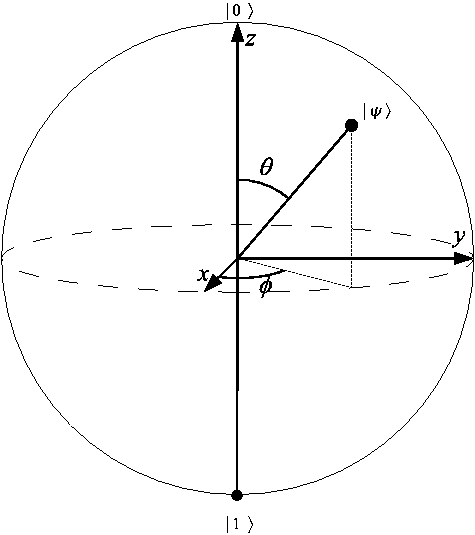
\includegraphics[scale=0.5]{Bloch.png}
\caption{The 1-Qubit Bloch Sphere \cite{QuantikiBlochSphereImage}}
\label{BlochSphere}
\end{figure}
A quantum state space can also been visualised in terms of the Bloch sphere, shown in Figure \ref{BlochSphere}.
The shown Bloch sphere is for a single qubit system, it can be extended to an n-qubit system however the visualisation breaks down.
All 'pure' quantum states can be described using the Bloch sphere and all exist on the surface produced by the unit sphere.
In this report only pure quantum states will be used and all explanation of quantum states are more precisely explanations of 'pure' quantum states.
This means that all superpositions of states can be expressed in terms of $|\psi\rangle = \cos \frac{\theta}{2} \, |0 \rangle +  e^{i \phi}  \sin \frac{\theta}{2}  \,|1 \rangle $ with $0 \leq \theta \leq \pi, \quad  0 \leq \phi \leq 2 \pi$, ignoring global phase factors\cite{BlochSphereTalk}.

In quantum mechanics, Kets are used to indicate a state, for example $\vert$0$\rangle$ is the state of a logical $0$ whereas $\vert$1$\rangle$ is the state of logical $1$.
Using this notation and the inclusion of probabilities, the state of the superposition can be expressed.

A dual to the Ket notation is the 'Bra' notation, $\langle$a$\vert$.
This notation is used to denote the 'dual vector' of the corresponding Ket.
For a state vector represented by
\begin{equation}\label{ket_explanation_example}
\vert
a
\rangle = 
\begin{pmatrix}
a_1\\
a_2\\
a_3\\
\vdots
\end{pmatrix}
\end{equation}
there is a dual vector representing its Hermitian conjugate
\begin{equation}\label{bra_explanation_example}
\langle
a
\vert = 
\begin{pmatrix}
a_1^*$$
a_2^*$$
a_3^*$$
\cdots
\end{pmatrix}
\end{equation}

Combining the two vectors $\langle$a$\vert$ and $\vert$b$\rangle$, written $\langle$a$\vert\vert$b$\rangle$, represents the inner product of the two vectors.
If a and b are unit vectors and $a == b$, $\langle$a$\vert\vert$b$\rangle == 1$.
If a and b are orthogonal, $\langle$a$\vert\vert$b$\rangle == 0$.

The outer product of two vectors, a and b, can be represented by $\vert$a$\rangle$$\langle$b$\vert$.
This represents the transformation from a to b.
It can also be represented in matrix form.

With
$\vert
0
\rangle
== 
\begin {pmatrix}
1\\
0\\
\end{pmatrix}
$
and
$\vert
1
\rangle
==  
\begin {pmatrix}
0\\
1\\
\end{pmatrix}
$
it is possible to represent $1$-qubit operations in the bra-ket notation.
For example, the NOT gate performs a simple negation of a qubit's value.
This can be written as $\vert0\rangle\langle1\vert + \vert1\rangle\langle0\vert$.
Substituting in the vector values we have
\begin{equation}
\begin{tabular}{ r c l }
\(\begin {pmatrix}
1\\
0
\end{pmatrix}
\begin {pmatrix}
0&&
1
\end{pmatrix}
 + 
\begin {pmatrix}
0\\
1
\end{pmatrix}
\begin {pmatrix}
1&&
0
\end{pmatrix}\)
& \(=\)
& \( 
\begin{pmatrix}
0 && 1 \\
0 && 0
\end{pmatrix}
 + 
\begin{pmatrix}
0 && 0\\
1 && 0
\end{pmatrix}
\) \\
& \(=\)
& \( 
\begin{pmatrix}
0 && 1 \\
1 && 0
\end{pmatrix}
\)
\end{tabular}
\label{eq:notexplanded}
\end{equation}

This matrix can be seen as a transformation matrix for the NOT operation.
In quantum computation, the NOT gate is one of the $4$ gates known as the Pauli gates, more specifically the Pauli-X gate.
It is called the Pauli-X gate as it can be seen as a rotation of $\pi$ radians about the X axis of the Bloch sphere, Figure \ref{BlochSphere}.

% Definition of Unitary
The matrices representing the Pauli-X gate and all other quantum logic gates are unitary.
A unitary matrix, U, is one which adheres to
\begin{equation}
U*{\dagger}
U == UU*{\dagger} = I_N
\end{equation}
where $I_N$ is the identity matrix in N dimensions and $U*{\dagger}$ is the complex conjugate of $U$.
% Reversible logic
The implication of all quantum logic operations being unitary is that they are reversible, this is a difference to classical computation.
With many classical logic gates irreversible, there is not a set of quantum logic gates which is as computationally powerful as the set of classical logic gates.
This seems like a major issue, quite the contrary.
The set of classical logic gates can be replaced by reversible equivalents and therefore it is possible to produce a set of quantum logic gates with the equivalent computational power as the classical logic gates.

%Superposition
As with all probabilities, the overall probability of a superposition collapsing to any of the states it contains must equal $1$.
\begin{equation}
\label{superposition_explanaiton}
\alpha\vert0\rangle+\beta\vert1\rangle
\end{equation}
\begin{equation}
\label{superposition_explanaiton_sum}
\frac{1}{2^{\frac{1}{n}}}\sum\limits_{i=0}^N \ket{x_i}
\end{equation}
Equation \eqref{superposition_explanaiton} is how the combination of the logical $0$ and $1$ states in a superposition can be represented for a single particle.
It can also be represented in the for of Equation \eqref{superposition_explanaiton}.
This is equivalent to the representation provided by the Bloch sphere, Figure \ref{BlochSphere}.
The probability of this state collapsing to the basis state $0$ can be calculated by $\vert\alpha\vert^2$ where $\alpha$ is a complex number.
$\alpha$ is known as the probability amplitude of $\vert0\rangle$.
Similarly, the probability of this state collapsing to the basis state $1$ can be calculated by $\vert\beta\vert^2$, $\beta$ being the probability amplitude of $\vert1\rangle$.
It follows that $\frac{1}{\sqrt{2}}\vert0\rangle+\frac{1}{\sqrt{2}}\vert1\rangle$ is an equal superposition where the collapse to 0 is just as likely as collapsing to $1$.
This provides the first glimpse of where a single qubit has the ability to perform a function not currently possible on a classical computer.
With n-qubits in the equal superposition, we have n binary values which have an equal probability of taking the value $0$ as the value $1$.
With an ordering decided of these qubits, collapsing the superposition of each qubit will result in a binary value of length n.
With all probabilities being $\frac{1}{2}$ this binary value takes a truly random value between $0$ and $2^n-1$.
It is not possible to produce a truly random number using a classical computer.

A second indication of the power held within the idea of superposition becomes clear if we look at the n-qubits in their equal superposition.
In 1935, Erwin Schr$\ddot{o}$ginger\cite{SchroedingersCat} proposed a thought experiment to explain the idea of superposition.
Imagine a cat in a fully opaque box with a vile of poison.
The vile may break at any time, a truly random variable.
After sealing the box the state of the cat is not known.
The cat could be alive if the vile has not broken but could just as likely be dead.
Only by looking inside the box will the state of the cat be known.
Until this time the cat could be thought of as both alive and dead at the same time.
If we assign 'dead' to the state $\vert0\rangle$ and 'alive' to the state $\vert1\rangle$ the situation looks very similar to the state we have previously seen.
Therefore, just as the cat can be thought of as both dead and alive at the same time, a qubit in the superposition $\frac{1}{\sqrt{2}}\vert0\rangle+\frac{1}{\sqrt{2}}\vert1\rangle$ can be thought of as both 0 and 1 at the same time.
This leads to a very powerful property of quantum computers.
With n classical bits, a single number in the range 0 to $2^n-1$ can be expressed at any one time.
With n quantum qubits, every number in the range 0 to $2^n-1$ can be expressed at any one time.
This effectively allows computation over the whole range of $2^n$ inputs to be carried out in parallel.

This parallelism is very powerful and has been shown to enable the computation of problems classified as NP to be performed in polynomial time.
This does however have a caveat.
As mentioned previously the superposition cannot itself be observed or measured.
When observed the superposition collapses to a basis state with respect to the superposition probability amplitudes.
This means that even though $2^n$ calculations can be performed in parallel, only a single answer can be observed.

% mathematic examples of matrices and the application
Along with the Pauli-X gate, there are an additional 3 Pauli gates.
The Pauli-I gate is the simplest of all quantum gates.
It is the identity gate, the output is identical to the input.
In Dirac notation this is $\vert0\rangle\langle0\vert + \vert1\rangle\langle1\vert$, and in matrix form below
\begin{equation}
\begin{tabular}{ r c l }
\(\begin {pmatrix}
1\\
0
\end{pmatrix}
\begin {pmatrix}
1&&
0
\end{pmatrix}
 + 
\begin {pmatrix}
0\\
1
\end{pmatrix}
\begin {pmatrix}
0&&
1
\end{pmatrix}\)
& \(=\)
& \( 
\begin{pmatrix}
1 && 0 \\
0 && 0
\end{pmatrix}
 + 
\begin{pmatrix}
0 && 0\\
0 && 1
\end{pmatrix}
\) \\
& \(=\)
& \( 
\begin{pmatrix}
1 && 0 \\
0 && 1
\end{pmatrix}
\)
\end{tabular}
\end{equation}

The Pauli-Z gate is similar to the Pauli-X gate, but differs in the axis about which it performs the rotation.
The Pauli-Z gate rotates the quantum state by $\pi$ radians about the Z axis.
This represents a phase flip of the quantum state.
The phase of a state is important when interference is used in computation.
In Dirac notation this is $\vert0\rangle
\langle0\vert + \vert1\rangle(-\langle1\vert$), and in matrix form below
\begin{equation}
\begin{tabular}{ r c l }
\(\begin {pmatrix}
1\\
0
\end{pmatrix}
\begin {pmatrix}
1&&
0
\end{pmatrix}
 + 
\begin {pmatrix}
0\\
1
\end{pmatrix}
\begin {pmatrix}
0&&
-1
\end{pmatrix}\)
& \(=\)
& \( 
\begin{pmatrix}
1 && 0 \\
0 && 0
\end{pmatrix}
 + 
\begin{pmatrix}
0 && 0\\
0 && -1
\end{pmatrix}
\) \\
& \(=\)
& \( 
\begin{pmatrix}
1 && 0 \\
0 && -1
\end{pmatrix}
\)
\end{tabular}
\end{equation}

The Pauli-Y gate is similar to both the Pauli-X and Pauli-Z gates, but differs in the axis about which it performs the rotation.
The Pauli-Y gate rotates the quantum state by $\pi$ radians about the Y axis.
This represents a phase flip followed by a bit flip.
In Dirac notation this is $\vert0\rangle
(i\langle1\vert) + \vert1\rangle(-i\langle0\vert$), and in matrix form below
\begin{equation}
\begin{tabular}{ r c l }
\(\begin {pmatrix}
1 \\
0
\end{pmatrix}
\begin {pmatrix}
0 &&
-i
\end{pmatrix}
 + 
\begin {pmatrix}
0 \\
1
\end{pmatrix}
\begin {pmatrix}
i &&
0
\end{pmatrix}\)
& \(=\)
& \( 
\begin{pmatrix}
0 && -i \\
0 && 0
\end{pmatrix}
 + 
\begin{pmatrix}
0 && 0\\
i && 0
\end{pmatrix}
\) \\
& \(=\)
& \( 
\begin{pmatrix}
0 && -i \\
i && 0
\end{pmatrix}
\)
\end{tabular}
\end{equation}

Along with the single qubit operations, like those above, there are operations which can act over n-qubits.
A simple example of a 2 qubit operation is the controlled-NOT, CNOT, operator.
This is a simple extension of the Pauli-X gate.
\begin{table}
\centering
\begin{tabular}{ l | c || r | }
0 & 0 & 0 \\
0 & 1 & 1 \\
1 & 0 & 1 \\
1 & 1 & 0 \\ \end{tabular}
\caption{Classical CNOT Truth Table}
\label{CNOTTruthTable}
\end{table}
The CNOT gate has a control input which it requires to be in the logical $1$ state for the NOT operation on the second input to be carried out.
In classical logic this would extend the truth table to be as shown in Table \ref{CNOTTruthTable}.
The truth table of the CNOT gate is the same as that of the XOR gate.
The Dirac notation of the CNOT gate is $\vert00\rangle\langle00\vert + \vert01\rangle\langle01\vert + \vert10\rangle\langle11\vert + \vert11\rangle\langle10\vert$.

\section{An Introduction to Quantum Algorithms}
%Known Quantum Algorithms

Just as with classical computers, the computation to produce the required output given inputs is given in the form of an algorithm.
Quantum algorithms can be constructed in several ways. These definitions are based on those provided by Massey\cite{masseythesis}.

\begin{itemize}
\item A quantum circuit can be used to represent an algorithm at the level of quantum logic gates.
This is similar to a specific purpose circuit diagram for classical systems.
\item A quantum program is a representation of the algorithm in some higher level quantum 'programming' language which would generate the required circuit.
The circuit generated is not defined in this method, just it's behaviour.
This could be seen as slightly more flexible that the quantum circuit model as the 'compiler' can be updated to reflect the findings of future research.
\item A parameterisable quantum algorithm is a representation in pure Pseudo-code.
It proves the flexibility of changing some value n, which is used to indicate the number of input qubits, to produce quantum circuits or programs with the desired behaviour on n qubits.
This is the most flexible construction of quantum algorithms.
It can cope with the changing in input size and can use findings of research just like in the 'compilation' of a quantum program.
\end{itemize}

Currently there are very few quantum algorithms known.
Peter Shor has carried out, and published, a discussion on the progress made `in discovering algorithms for computation on a quantum computer`\cite{Shor:2004:PQA:1032132.1032149}.
Shor suggests two possible reasons for the lack of quantum algorithms.
The first is `that there might really be only a few problems for which quantum computers can offer a substantial speed-up over classical computers`\cite{Shor:2004:PQA:1032132.1032149}.
This would indeed make the discovery of useful quantum algorithms difficult.
However, I feel this is somewhat pessimistic.
The main focus of the paper published by Feynman\cite{Feynman82simulatingphysics} was the problem of simulating the physics of quantum mechanics on a classical computer.
This to suggests there would be the potential of many applications of quantum computers, even if they aren't analogous to the classical computational applications.

The second is `that quantum computers operate in a manner so non-intuitive, and so different from classical computers`\cite{Shor:2004:PQA:1032132.1032149} that our current algorithm knowledge is close to useless.
This, in my opinion, is a much more believable obstacle.
Quantum mechanics is seen by many as a confusing and mystical subject.
Even prize winning mathematician and physicist Roger Penrose is attributed to the remark `Quantum mechanics makes absolutely no sense`.
Statements like this and the atmosphere surrounding quantum mechanics makes the potential of its study more than some what daunting.
As computer scientists, the exposure to and therefore our understanding of quantum mechanics is limited, in general.
With this in mind it is, currently, unreasonable to expect the discovery of algorithms that exploit the finer details of this complex and subtle theory to become an everyday occurrence.

The following few sections outline a selection of the currently known quantum algorithms.

\subsection{Deutsch Algorithms}
\label{sec:DeutAlg}
The original Deutsch algorithm\cite{Deutsch1985} was proposed to solve the following problem:
\begin{quote}
Given a function $f:\{0,1\}\to\{0,1\}$, decide whether it is either a balanced, or constant function.
The function $f(x)$ is guaranteed to be either constant or balanced.
\end{quote}
The algorithm's major breakthrough was that it only required a single invocation of the function $f(x)$ to decide on which category it belonged.
This is compared to the best classical approach requiring $2$ invocations to the function.
This was the first algorithm that it was possible to compute the solution to a problem, provably, more efficiently than a classical computer by exploiting quantum mechanics.

\begin{figure}
\[
\Qcircuit @C=1.0em @R=.7em {
& \lstick{\ket{0}} & \gate{H} & \gate{\mathcal{F}} & \gate{H} & \measure{meas} \\
& \lstick{\ket{1}} & \gate{H} & \targ\qwx & \rstick{\ket{0}-\ket{1}}\qw  
}
\]
\caption{Deutsch Circuit}
 \label{Deutsch-Cir}
\end{figure}

The circuit for this algorithm is presented in Figure \ref{Deutsch-Cir}.
The maths for the way in which the state evolves is below
\begin{equation}
\ket{01} \xrightarrow{H\otimes{H}} \frac{1}{\sqrt{2}}(\ket{0}+\ket{1})\frac{1}{\sqrt{2}}(\ket{0}-\ket{1})
\end{equation}

 Using the identity $(\ket{b}-\ket{a})\equiv-1(\ket{a}-\ket{b})$, if $f(x)$ evalues to $0$ the state transformation is
\begin{equation*}
 \ket{x}\frac{1}{\sqrt{2}}(\ket{0}-\ket{1}) \xrightarrow{f} \ket{x}\frac{1}{\sqrt{2}}(\ket{0}-\ket{1})
\end{equation*}
Wheras if $f(x)$ evaluates to $1$ the state transformation is
\begin{equation*}
 \ket{x}\frac{1}{\sqrt{2}}(\ket{0}-\ket{1}) \xrightarrow{f} -\ket{x}\frac{1}{\sqrt{2}}(\ket{0}-\ket{1})
\end{equation*}
These two equations can be generalised to give
\begin{equation*}
 \ket{x}\frac{1}{\sqrt{2}}(\ket{0}-\ket{1}) \xrightarrow{f} (-1)^{f(x)}\ket{x}\frac{1}{\sqrt{2}}(\ket{0}-\ket{1})
\end{equation*}
This is due to $(-1)^0=1$ and $(-1)^1=-1$ which is the way the state evolves with the outputs of $f(x)$.
Using this we can continue to analyse how the state evolves for the superposition $\frac{1}{\sqrt{2}}(\ket{0}+\ket{1})\frac{1}{\sqrt{2}}(\ket{0}-\ket{1})$.
\begin{equation*}
 \frac{1}{\sqrt{2}}(\ket{0}+\ket{1})\frac{1}{\sqrt{2}}(\ket{0}-\ket{1}) \xrightarrow{f} \frac{1}{\sqrt{2}}((-1)^{f(0)}\ket{0}+(-1)^{f(1)}\ket{1})\frac{1}{\sqrt{2}}(\ket{0}-\ket{1})
\end{equation*}
\begin{equation*}
 \frac{1}{\sqrt{2}}((-1)^{f(0)}\ket{0}+(-1)^{f(1)}\ket{1})\frac{1}{\sqrt{2}}(\ket{0}-\ket{1}) \equiv (-1)^{f(0)}\frac{1}{\sqrt{2}}(\ket{0}+(-1)^{f(0)\oplus{f(1)}}\ket{1})\frac{1}{\sqrt{2}}(\ket{0}-\ket{1})
\end{equation*}
This penultimate state, before the last hadamard, can be simplified.
Global phase factors cannot be observed so the $(-1)^{f(0)}$ can be ignored.
The second qubit can also be ignored as it is not entangled with the first, nor is it ever measured.
\begin{equation}
 \frac{1}{\sqrt{2}}(\ket{0}+(-1)^{f(0)\oplus{f(1)}}\ket{1})
\label{Deutsch_final_state}
\end{equation}
This results in the penultimate state being able to be represented as \ref{Deutsch_final_state}.
With this as the state we can reason about the output if the function $f(x)$ is balanced and if it is constant.
If f were balanced, $f(0) \oplus f(1) = 1$ due to either $f(0)$ or $f(1)$ evaluating to $1$ but not both.
If f were constant, $f(0) \oplus f(1) = 0$ due to either $f(0)$ and $f(1)$ both evaluating to $0$ or both evaluating to $1$.
Using these two observations we can see the penultimate state, \ref{Deutsch_final_state}, when f is constant and when f is balanced.
When f is balanced $\frac{1}{\sqrt{2}}(\ket{0}+(-1)^{f(0)\oplus{f(1)}}\ket{1}) \equiv \frac{1}{\sqrt{2}}(\ket{0}-\ket{1})$.
When this is passed through the final hadamard $\frac{1}{\sqrt{2}}(\ket{0}-\ket{1}) \xrightarrow{H} \ket{1}$.
When f is constant $\frac{1}{\sqrt{2}}(\ket{0}+(-1)^{f(0)\oplus{f(1)}}\ket{1}) \equiv \frac{1}{\sqrt{2}}(\ket{0}+\ket{1})$.
However, when this is passed through the final hadamard $\frac{1}{\sqrt{2}}(\ket{0}+\ket{1}) \xrightarrow{H} \ket{0}$.
This means that using just a single query to the function $f(x)$, the algorithm can provide an answer to the problem.


\subsection{Deutsch-Jozsa Algorithm}
%Deutsch-Jozsa Algorithm
The Deutsch-Jozsa algorithm\cite{1992-deutsch} is a generalisation and improvement over an earlier Deutsch algorithm\cite{Deutsch1985}.
The algorithm described here will be the algorithm including the improvements published in \cite{Macchiavello97quantumalgorithms}, the resulting algorithm is still referred to as the Deutsch-Jozsa algorithm.

In 1992, David Deutsch and Richard Jozsa\cite{1992-deutsch} presented an extension to the Deutsch algorithm, Section \ref{sec:DeutAlg}, that allowed for functions $f:\{0,1\}^{2n}\to\{0,1\}$ to be categorised as constant or balanced.
The algorithm was probabilistic but also required 2 invocations to the function $f(x)$.
This means that in the worst case, with $f_1:\{0,1\}\to\{0,1\}$, the algorithm will perform worst than both the original Deutsch algorithm\cite{Deutsch1985} and the classical algorithm due to the probabilistic nature of its result.
This is a very limited case and performance improves as the value of n increases.
As with the original algorithm, the number of invocations of $f(x)$ is constant, truly independent of both $n$ and $f(x)$.
This is again an improvement over the classical algorithm which requires in the worst case $2^{n-1}+1$ to be certain of the function's classification.
\begin{figure}
\[
\Qcircuit @C=1.0em @R=.7em {
& \lstick{\ket{0}} & \gate{H} & \multigate{3}{\mathcal{F}} & \gate{H} & \measure{meas} \\
& \lstick{\ket{0}} & \gate{H} & \ghost{\mathcal{F}} & \gate{H} & \measure{meas} \\
& \lstick{\ket{0}} & \gate{H} & \ghost{\mathcal{F}} & \gate{H} & \measure{meas} \\
& \lstick{\ket{0}} & \gate{H} & \ghost{\mathcal{F}}  & \gate{H} & \measure{meas} \\
& \lstick{\ket{1}} & \gate{H} & \targ\qwx & \rstick{\ket{0}-\ket{1}}\qw   
}
\]
\caption{Deutsch-Jozsa Circuit}
 \label{Deutsch-Jozsa-Cir}
\end{figure}

The algorithm requires n input qubits and a single control qubit.
The n input qubits are initialised to $\ket{0}$.
The control qubit is initialised to $\ket{1}$.
The n-fold Hadamard gates are then used to produce the superposition of all $0..2^n-1$ possible inputs, $x=(\ket{0}+\ket{1})^n$.
The Hadamard gate on the control qubit is used to produce the superposition $\ket{0}-\ket{1}$.
The difference in superpositions between the input and control qubits is important to the way in which the algorithm classifies a function.
This produces a state  $(\ket{0}+\ket{1})^n(\ket{0}-\ket{1})$.

% The n input qubits, in the superposition $(\ket{0}+\ket{1})^n$, are then passed to the function we wish to classify, $f(x)$.
The result of $f(x)$ is used as the control for a CNOT gate acting on the control qubit.
Remember at this point that the input x is in effect all possible inputs to $f(x)$, and as such the output is all the respective outputs.
This means that each of the factors of the input are transformed, based on the action of $f(x)$.
This can be formalised as $U_f(\ket{x},\ket{y})=(\ket{x},\ket{f(x)\oplus{y}})$.
Using the final Hadamard gates we can use the transformation to categorise $f(x)$.

If we assume n to be equal to 2, then after the initial Hadamard gates we have the superposition:
\begin{equation*}
\frac{1}{2}\ket{\Psi_{init}}\frac{1}{\sqrt{2}}(\ket{0}-\ket{1})=\frac{1}{2}(\ket{00}+\ket{01}+\ket{10}+\ket{11})\frac{1}{\sqrt{2}}(\ket{0}-\ket{1})
\end{equation*}
\begin{equation}
\ket{a}(\ket{c}-\ket{b})\equiv\ket{a}(-1(\ket{b}-\ket{c}))\equiv-1\ket{a}(\ket{b}-\ket{c})
\label{target_qubit_identity}
\end{equation}
The CNOT on the target qubit is only activated if $f(x)=1$ which, using the equivalent above, produces the superposition $-1(\ket{0}-\ket{1})$.
This can also be generalised as $(-1)^{f(x)}(\ket{0}-\ket{1})$ where $-1^1=-1$ and $-1^0=1$ by definition.
By linearity the superposition after the CNOT controlled by f(x) on the target qubit becomes
\begin{equation*}
\frac{1}{2}((-1)^{f(00)}\ket{00}+(-1)^{f(01)}\ket{01}+(-1)^{f(10)}\ket{10}+(-1)^{f(11)}\ket{11})\frac{1}{\sqrt{2}}(\ket{0}-\ket{1})
\end{equation*}

After the application of $f(x)$, the target bit has served it purpose and is neither measured nor entangled with any of the qubits from the n qubit input.
To simplify the equations I will now ignore the $(\frac{1}{\sqrt{2}}\ket{0}-\ket{1})$ contributed by the target qubit, the remaining state will be refereed to as $\Psi$.
If the function $f(x)$ is constant:
\begin{equation*}
\ket{\Psi_{const}}=\pm\frac{1}{2}(\ket{00}+\ket{01}+\ket{10}+\ket{11})
\end{equation*}
Whereas if $f(x)$ is balanced then:
\begin{equation*}
\ket{\Psi_{bal}}=(-1)^{f(00)}\ket{00}+(-1)^{f(01)}\ket{01}+(-1)^{f(10)}\ket{10}+(-1)^{f(11)}\ket{11}
\end{equation*}
However,as $\ket{\Psi_{const}}$ and $\ket{\Psi_{bal}}$ are orthogonal we can use this to detect if the function is balanced or constant.
\begin{equation*}
\bra{\Psi_{bal}}\ket{\Psi_{const}} = 0
\end{equation*}

Applying the n Hadamard gates to the state $\Psi_{const}$ produces the state $\pm\ket{0}^n$.
When measured this will return the result $0$ as the global phase factor $\pm$ cannot be observed.
As we have noted, $\Psi_{const}$ is orthogonal to $\Psi_{bal}$ so when the n Hadamard gates are applied, as they preserve orthogonality, the measured result will be anything orthogonal to $0$.
This gives us a clear way of distinguishing between whether f is constant of balanced with certainty and only a single invocation of f.
If the measurement returns $0$ then $f(x)$ is constant, if the measurement returns anything else $f(x)$ is balanced.

\subsection{Grover's Search Algorithm}	
%Grovers Database search algorithm
The Grover Search algorithm\cite{Grover:1996rk} is an unstructured search problem.
The algorithm assumes no underlying structure in the search space.
By this I mean the algorithm does not exploit, and therefore assume, any structure, such as sorting, in the data set being searched.

It has previously been proven\cite{Bennett:1996iu} that the lower complexity limit for any algorithm identifying an element without knowledge of underlying structure in the data is $\Omega(\sqrt{N})$.
For simplicities sake we assume $N=2^n$.
The complexity is measured by the number of elements which need to be queried in order to find the desired element.
The Grover Search algorithm has the complexity $O(\sqrt{N})$ and so `is within a constant factor of the fastest possible quantum mechanical algorithm`\cite{Grover:1996rk}.

\begin{figure}
\[
\Qcircuit @C=1.0em @R=.7em {
& \qw 		& \qw 	& \multigate{3}{f} 	&\qw 	&  \gate{H} 	&\qw 	& \multigate{3}{f_0} 	&\qw &  \gate{H}  	&\qw 	&\qw\\
& \vdots 	& 	&  \ghost{f} 		& \qw 	& \vdots 	& 	& \ghost{f_0} 		&\qw &  \vdots 		& 	&\qw\\
& \vdots 	& 	& \ghost{f} 		& \qw 	& \vdots 	& 	& \ghost{f_0} 		&\qw &  \vdots 		& 	&\qw\\
& \qw 		&\qw 	&  \ghost{f} 		& \qw 	& \gate{H} 	&\qw 	& \ghost{f_0} 		&\qw &  \gate{H} 	&\qw 	&\qw\\
& \qw 		&\qw 	&  \targ \qwx 		&\qw 	&  \qw 		&\qw 	& \targ \qwx 		&\qw &  \gate{X} 	&\qw	&\qw 
}
\]
\caption{Grover's Search Circuit}
 \label{Grovers-Search-Cir}
\end{figure}


The mechanisms used within the algorithm to produce a solution to the problem is more subtle than those used but the Deutsch-Jozsa algorithm.
The algorithm does not perform the computation in a single step.
The algorithm requires $O(\sqrt{N})$ steps.
The section of circuit which is repeated is that shown in Figure \ref{Grovers-Search-Cir}.

The algorithm is to initialise the state, $\Psi_1$, using n Hadamard gates.
\begin{equation*}
\Psi_1=\frac{1}{2^{\frac{1}{n}}}\sum\limits_{i=0}^N \ket{x_i}(\ket{0}-\ket{1})
\end{equation*}
The application of $f(x)$ is used in an analogous way to in the Deutsch-Jozsa algorithm.
It can again be written as $U_f(\ket{x},\ket{y})=(\ket{x},\ket{f(x)\oplus{y}})$ and remember
\begin{equation*}
 \exists{x_i}\epsilon\{x_0,x_1,\ldots,x_{n-1}\}|f(x_i)=1
\end{equation*}
\begin{equation*}
\forall{x_j} : i\neq{j} : f(x_j)=0
\end{equation*}
Just as in the Deutsch-Jozsa algorithm, the result of a $1$ produces a bit flip on the target qubit.
Using the identity in Equation \ref{target_qubit_identity} this flips the sign on the amplitude associated with $x_i$, where $f(x_i)=1$.
The state $\Psi_1$ is transformed by $U_f$ to $\Psi_2$.
\begin{equation*}
\Psi_2=\frac{1}{2^{\frac{1}{n}}}\sum\limits_{j=0\wedge{j}\neq{i}}^N \ket{x_j}(\ket{0}-\ket{1}) - \frac{1}{2^{\frac{1}{n}}} \ket{x_i}(\ket{0}-\ket{1})
\end{equation*}
The second function in the circuit, $f_0(x)$, is a fixed function.
It is not dependant on $f(x)$ but is a function which evaluates to $1$ only when the input is $\ket{0}$.
This means that given a simple state $(\alpha\ket{0}+\beta\ket{1}+\ldots)$ the result is the state $(-\alpha\ket{0}+\beta\ket{1}+\ldots)$.
The action of both these function can be written in the shorter and much simpler Dirac notation.
\begin{equation*}
U_f=I-2\ket{x_i}\bra{x_i}
\end{equation*}
\begin{equation}
U_0=I-2\ket{0}\bra{0}
\label{Grover:U_0_dirac}
\end{equation}

Functions $f(x)$ and $f_0(x)$ seem relatively unimpressive and don't appear to solve the problem.
The importance of the two sets of n Hadamard gates, one each side of $f_0(x)$, is paramount.
The effect they have on the action of $f_0(x)$ is shown below, the action of $f_0(x)$ and the Hadamard gates will be represented as V.
\begin{equation*}
V=H^{\otimes{n}}U_0{H}^{\otimes{n}}
\end{equation*}
\begin{equation*}
V=H^{\otimes{n}}(I_n-2\ket{0}\bra{0}){H}^{\otimes{n}}
\end{equation*}
\begin{equation*}
V=H^{\otimes{n}}I_n{H}^{\otimes{n}}-H^{\otimes{n}}(2\ket{0}\bra{0}){H}^{\otimes{n}}
\end{equation*}
\begin{equation*}
V=I_n-2(H^{\otimes{n}}\ket{0})(\bra{0}{H}^{\otimes{n}})
\end{equation*}
\begin{equation*}
V=I_n-2(H^{\otimes{n}}\ket{0})({H}^{\otimes{n}}\ket{0})^\dagger
\end{equation*}
The application of Hadamard gates to the $\ket{0}$ state is the method of creating the superposition of all $2^n-1$ possible states.
\begin{equation*}
V=I_n-2(\frac{1}{2^{\frac{1}{n}}}\sum\limits_{i=0}^N \ket{x_i})(\frac{1}{2^{\frac{1}{n}}}\sum\limits_{i=0}^N \ket{x_i})^\dagger
\end{equation*}
\begin{equation*}
V=I_n-2(\frac{1}{2^{\frac{1}{n}}}\sum\limits_{i=0}^N \ket{x_i})(\frac{1}{2^{\frac{1}{n}}}\sum\limits_{i=0}^N \bra{x_i})
\end{equation*}
\begin{equation*}
V=I_n-2\ket{\Psi}\bra{\Psi}
\end{equation*}
Just as with $U_f$, V can be seen as a simple phase flip.
However, the subtlety of this operator is that the flip is not in the computational basis, but in the basis described by $\ket{\Psi}$.

The last gate in Figure \ref{Grovers-Search-Cir} is the Pauli-X operator.
This is not functional but for convenience of mathematics as produces a global phase flip of $\ket{\Psi}$ which makes the mathematics simpler.

That is Grovers algorithm.
Looking at the circuit and the mathematics of the operators it doesn't provide an obvious answer as to how it solves the search problem.
This is partly due to the fact the circuit in Figure \ref{Grovers-Search-Cir} has to be repeated roughly $\frac{\pi\sqrt{N}}{4}$ times and partly due to the effect of the circuit being hidden in implementation.
The circuit is actually little more than a complex rotation gate.
It is however more sophisticated than a standard rotation gate as it computes the direction to rotate the state so as to solve the problem.
The power of this does not initially appear as immense as it possibly should.
The Hilbert space in which this circuit is operating is of the order $N$, we as humans can only accurately imagine a maximum of a $3$ dimensional space as it the most dimensions we can observe directly.
Taking into account the vast Hilbert space when assessing this circuit produces a much better appreciation its power.

However, even though the power can now be appreciated, the way in which it solves the problem is still not clear. 

\subsection{Shor's Factorisation Algorithm}
%Shors Algorithm
In 1994, Peter Shor astonished the computer science community with a quantum factorisation algorithm\cite{Shor:1994jg}.
This allowed the factorisation of integers into their constituent primes in polynomial time.
This algorithm is not a pure quantum algorithm, but a hybrid algorithm.
It has both a quantum and classical portion.

The algorithm utilises the complex nature of the probability amplitudes.
This means that the relative phase of the states is important.
To explain Shors algorithm it is necessary to introduce the sum of complex roots of unity.

\begin{equation}
 \sum_{j=0}^{N-1}z^j=\frac{1-z^N}{1-z}
\label{sumofpowers}
\end{equation}

Equation \ref{sumofpowers} provides a simplification of the sum of the geometric series $\sum_{j=0}^{N-1}z^j$.
This simplification can be applied to both real and complex values of z, including the roots of unity.
Taking $w=e^{\frac{2\pi{i}}{N}}$ to be the N-th root of unity, the geometric series $\sum_{i=0}^{N-1}w^{xy}$ can be simplified using Equation \ref{sumofpowers}.

When $x=0$
\begin{equation}
 \sum_{y=0}^{N-1}w^{xy}=\sum_{y=0}^{N-1}w^{0}=\sum_{y=0}^{N-1}1 = N
\end{equation}
However, when $x\neq{0}$
\begin{equation}
 \sum_{y=0}^{N-1}w^{xy}=\sum_{y=0}^{N-1}(w^x)^y=(\frac{1-w^N}{1-w})^y=0^y=0
\end{equation}
The result of this is generally described using a Kronecker delta
\begin{equation}
 \sum_{y=0}^{N-1}w^{xy}=N\times\delta_{x,y}=N\times
\left\{
  \begin{array}{cc} 1, & \mbox{if } x={0}\\ 
  0, & \mbox{if } x\neq{0}\end{array}
\right.
\label{krondelt}
\end{equation}

This produces a very neat and convenient explanation of such a series.
As the sum is of a root of unity raised to a power, it is a periodic function $w^0=w^N=1$.
This holds true in Equation \ref{krondelt} when $x=0,\pm{N},\pm{2N},\dots$.
With this the Kronecker delta can be expressed in terms of modular arithmetic.
\begin{equation}
 \sum_{y=0}^{N-1}e^{\frac{2\pi{i}xy}{N}}=N\times\delta_{x,y (mod N)}=N\times
\left\{
  \begin{array}{cc} 1, & \mbox{if } x={0}\\ 
  0, & \mbox{if } x\neq{0}\end{array}
\right.
\label{krondelt}
\end{equation}

The quantum section of Shor's algorithm is a period finding function.
The classical part then uses this period and number theory to deduce the factors.
In the explaination below, the value that is trying to be factorised is $N$ and the value $M$ is a value which is larger than $N$.
The use of the Kronecker delta, and understanding on the effect it has is vital to the explanation of the quantum section of Shor's algorithm.

\begin{figure}
\[
\Qcircuit @C=1.0em @R=.7em {
&\ket{0}&	& \qw	&\multigate{3}{\mathcal{F}^{-1}_M}	& \qw 	&\multigate{3}{f}	&\qw &\multigate{3}{\mathcal{F}_M}	&\qw	& \qw 	& \qw 	&\qw\\
&\vdots	&	&	&\ghost{\mathcal{F}^{-1}_M} 		&\qw 	&\ghost{f}		&\qw &\ghost{\mathcal{F}_M}		&	&\vdots & 	&\qw\\
&\vdots	&	&	&\ghost{\mathcal{F}^{-1}_M} 		&\qw 	&\ghost{f}		&\qw &\ghost{\mathcal{F}_M}		&	&\vdots & 	&\qw\\
&\ket{0}&	&\qw	&\ghost{\mathcal{F}^{-1}_M} 		&\qw 	&\ghost{f}		&\qw &\ghost{\mathcal{F}_M}		&\qw	&\qw 	&\qw	&\qw\\
&\ket{0}&	&\qw	&\qw 					&\qw 	&\multigate{3}{+}\qwx	&\qw &\qw 				&\qw	&\qw 	&\qw	&\qw\\
&\vdots	&	&	&\vdots 				&	&\ghost{+}		&\qw &\vdots 				&	&\vdots	&	&\\
&\vdots	&	&	&\vdots 				&	&\ghost{+}		&\qw &\vdots 				&	&\vdots	&	&\\
&\ket{0}&	&\qw	&\qw 					&\qw	&\ghost{+}		&\qw &\qw 				&\qw	&\qw	&\qw 	&\qw    
}
\]
\label{shorcirc}
\caption{The circuit of Shor's algorithm}
\end{figure}

The circuit in Figure \ref{shorcirc} is the period finding section of Shor's Algorithm.
The function $f$ is a periodic function, whose period we want to find.
$\mathcal{F}$ and $\mathcal{F}^{-1}$ are the Quantum Fourier Transform and the inverse, respectively.
\begin{equation}
 \mathcal{F}_N\ket{x}=\frac{1}{\sqrt{N}}\sum_{y=0}^{N-1}e^{\frac{2\pi{i}xy}{N}}\ket{y}
\label{QFTeq}
\end{equation}
\begin{equation}
 \mathcal{F}^{-1}_N\ket{y}=\frac{1}{\sqrt{N}}\sum_{z=0}^{N-1}e^{\frac{-2\pi{i}xy}{N}}\ket{z}
\label{QFTInveq}
\end{equation}

The action of applying the Quantum Fourier Transform and the inverse can be seen in Equations \ref{QFTeq} and \ref{QFTInveq} respectively.

The way in which this circuit computes the period is not initially apparent.
The central section of the circuit, involving the periodic function, performs the operation $U_f\ket{x}\ket{y}=\ket{x}\ket{f(x)+y}$ in the computaional basis.
However, it is preceded by the inverse Quantum Fourier Transform.
The application of the inverse Quantum Fourier Transform on the initial state is as follows:

\begin{equation*}
 \ket{0}\ket{0} \rightarrow \frac{1}{\sqrt{M}}\sum_{x=0}^{M-1}e^{\frac{-2\pi{i}x.0}{M}\ket{x}\ket{0}}
\end{equation*}
\begin{equation*}
 \frac{1}{\sqrt{M}}\sum_{x=0}^{M-1}\ket{x}\ket{0}
\end{equation*}

This produces a uniform superposition, just as a series of Hadamard gates would have produced.
The application of $f(x)$ to this superposition produces the state:
\begin{equation*}
 \frac{1}{\sqrt{M}}\sum_{x=0}^{M-1}\ket{x}\ket{f(x)}
\end{equation*}
Applying the final Quantum Fourier Transform manipulates this state quite substantially.
\begin{equation}
 \frac{1}{\sqrt{M}}\sum_{x=0}^{M-1}\ket{x}\ket{f(x)} \rightarrow \frac{1}{M}\sum_{y=0}^{M-1}\sum_{x=0}^{M-1}e^{\frac{2\pi{i}xy}{M}}\ket{y}\ket{f(x)}
\label{QFTfinstate}
\end{equation}
The final state is Equation \ref{QFTfinstate}.
This does not initially appear particularly useful or interesting.
However, remembering that $f(x)$ is periodic, we can separate and analyse a single branch of the superposition.
With $f(x)=f(x+r)=f(x+2r)\dots$ where $r$ is the period of $f(x)$ the amplitude of the branch $\ket{y}\ket{f(x)}$ , with $x=x_0+mr for x=0,1,\dots,\frac{M}{r}-1$, can be written as:
\begin{equation*}
 \frac{1}{M}\sum_{m=0}^{\frac{M}{r}-1}e^{\frac{2\pi{i}(x_0+mr)y}{M}}\ket{y}\ket{f(x_0)}
\end{equation*}

This initially still does not look particularly interesting or useful when we are trying to find the period of $f(x)$.
However, with some rearragement this state can be expressed as:
\begin{equation}
 \frac{1}{M}e^{\frac{2\pi{i}x_0y}{M}}\sum_{m=0}^{\frac{M}{r}-1}e^{\frac{2\pi{i}my}{\frac{M}{r}}}\ket{y}\ket{f(x_0)}
\end{equation}
This contains a structure which was introduced with the sumation of roots of unity, \ref{sumofpowers}.
Using this observation, the $\sum_{m=0}^{\frac{M}{r}-1}e^{\frac{2\pi{i}my}{\frac{M}{r}}}$ section of the amplitude for the state $\ket{y}\ket{f(x_0)}$ is simplified to:
\begin{equation}
 \sum_{m=0}^{\frac{M}{r}-1}e^{\frac{2\pi{i}my}{\frac{M}{r}}}=\frac{M}{r}\delta_{y,0 (Mon\frac{M}{r})}=\frac{M}{r}
\left\{
  \begin{array}{cc} 1, & \mbox{if } y={0} (mod\frac{M}{r})\\ 
  0, & \mbox{otherwise}\end{array}
\right.
\end{equation}
With this simplifcation in place it can be seen that the probability amplitude of any branch where $y\neq{x}(mod\frac{M}{r})$ will be zero simply due to the Kronecker delta.
This results in the only branches with non-zero amplitudes being where $y=0,\frac{M}{r},\frac{2M}{r},\dots$ and so when the first input register is measured the state observed will be $\ket{\frac{kM}{r}}$.
After several repeats of the algorithm the value of $r$ can be deduced from the observed states.

To see how knowing the period can help factorise the number $N$ we analyse the function $f(x)=a^x(mod N)$.
This function is obviously periodic as it is modulo N.
With the period r, $a^r=1(mod N)$.
The value of $r$ will depend on the value of $a$.
Only the even values of $r$ are useful, if an odd value is found the value of $a$ should be changed and the new $r$ found.

When $r$ is even, $a^r=1(mod N) \rightarrow a^r-1=0(mod N) \rightarrow (a^r+1)(a^r-1)=0(mod N)$.
Once we have the equation in this form, we can use the values of $a^r+1)$ and $(a^r-1)$ separately as one of them, possibly both, with have a factor in common with $N$.
This can simply be found using the Chinese remainder theorm.

The advantage of Shor's algorithm is that the value of $r$ can be found much faster with all values of $x$ up to the limit of $M-1$ tested simultaneously.

\subsection{Quantum Teleportation Protocol}

The quantum teleportation protocol provides a solution to the problems
\begin{center}
Alice has a quantum state, $\ket{\Psi}$, which she wishes to send to Bob.
There is only a classical communication channel by which Alica and Bob can communicate.
\end{center}

With a classical state this would not be an issue.
Measurements on the different parts of that state Alice want to sent to Bob would be made, and these would then be communicated down the channel for Bob to replicate.
Unfortunately this is not possible for quantum states.
Quantum computation exploits the power of quantum mechanics, however quantum mechanics has its own caveats.

The ``No Cloning Theorm'' in the field of quantum computation is the results of quantum mechanic's ``Uncertainty Principle''.
The ``Uncertainty Principle'' states that ``that
the values of a pair of canonically conjugate observables such as position and momentum cannot both
be precisely determined in any quantum state''\cite{uncerth}.
Essentially this means that an unknown quantum state cannot be reproduced.

The classical approach is also halted by Holevo's Theorem.
This theorem states that from any $n$ qubit state, at most $n$ bits of classical information can be observed.
With a one qubit state, $\alpha\ket{0}+\beta\ket{1}$, the value of $\alpha$ and $\beta$ are required for the state to be reproduced.
The each of these require 2 values as they are complex numbers, 4 values in total.
The state can be rewriten to give $|\alpha|e^{i\theta_0}\ket{0}+|\beta|e^{i\theta_1}\ket{1}$.
As global phase factors cannot be observed it can be simplified to $|\alpha|\ket{0}+|\beta|e^{i\phi}\ket{1}$
This leaves the real values $|\alpha|, |\beta| and \psi$, down to 3 values.
We know that $|\alpha|^2+|\beta|^2=1$ so the value of $|beta|$ is can be calculated from the value of $|\alpha|$.
This leave just two values to specify.
However, both of these two values can be specified to any arbitary precision, requiring an arbitary number of bits of data.
As Holevo's Theorem limits the observable information to just a single bit, for the one qubit state, the measure and recreate approach is impossible.

After stating these two theorems, the problem Alice and Bob face seems impossible.
However, there are subtleties to the laws governing quantum mechanics which actually make it possible, with a few concessions.

For Alice to sent the state $\ket{Phi}$, $\alpha\ket{0}+\beta\ket{1}$, the protocol is as follows:
\begin{itemize}
 \item Alice and Bob share the entangled state $\frac{1}{\sqrt{2}}\ket{00}+\frac{1}{\sqrt{2}}\ket{11}$.
This results in the state, the subscript letters are to show who is in possession of which qubits:
\begin{equation}
 \frac{1}{\sqrt{2}}(\alpha\ket{00}_A\ket{0}_B+\beta\ket{10}_A\ket{0}_B+\alpha\ket{01}_A\ket{1}_B+beta\ket{11}_A\ket{1}_B)
\end{equation}
\item Alice takes a measurement in the Bell Basis.
The Bell basis is a basis set which are not orthogonal to the computational basis.
This means that the measurement does not collapse the state.
The Bell basis vectors are $\ket{00}+\ket{11}, \ket{00}-\ket{11}, \ket{01}+\ket{10} and \ket{01}-\ket{10}$.
\begin{center}
\begin{tabular}{cc}
Alice measures & Remaining state\\
$\ket{00}_A+\ket{11}_A$ & $\alpha\ket{0}_B+\beta\ket{1}$\\
$\ket{00}_A-\ket{11}_A$ & $\alpha\ket{0}_B-\beta\ket{1}_B$\\
$\ket{01}_A+\ket{10}_A$ & $\alpha\ket{1}_B+\beta\ket{0}_B$\\
$\ket{01}_A-\ket{10}_A$ & $\alpha\ket{1}_B-\beta\ket{0}_B$
\end{tabular}
\end{center}

\item Based on the measurement Alice make she can instruct Bob, using the classical communication channel, to perform certain operations to change the remaining state into the original state $\ket{\Psi}$.
\begin{center}
\begin{tabular}{cc}
Remaining state & Bob applies to produce $\ket{\Psi}$\\
$\alpha\ket{0}_B+\beta\ket{1}_B$ & Nothing\\
$\alpha\ket{0}_B-\beta\ket{1}_B$ & Phase Flip\\
$\alpha\ket{1}_B+\beta\ket{0}_B$ & Bit Flip\\
$\alpha\ket{1}_B-\beta\ket{0}_B$ & Bit Flip followed by a Phase Flip
\end{tabular}
\end{center}
\end{itemize}

At the end of this protocol, the state $\ket{\Psi}$ has be teleported to Bob.
However, this must not violate either the No Cloning Theorem or Holevo's Theorem.
The No Cloning Theorem is not violated as to teleport the state to Bob, Alice must destroy her copy of $\ket{\Psi}$.
This means that at no point are there two copies of $\ket{\Psi}$, therefore does not violate the No Cloning Theorm.
The protocol does not violate Holevo's Theorem as at no point is any data observed from the state.
The true identity and nature, the probability amplitues, of the state $\ket{\Psi}$ is never known.

The circuit to implement the quantum teleportation protocol can be seel in Figure \ref{quantelcir}.

\begin{figure}
\[
\Qcircuit @C=.7em @R=.4em @! {
\lstick{\ket{\psi}} & \qw & \qw & \ctrl{1} & \gate{H} & \meter & \control \cw\\
\lstick{\ket{0}} & \qw & \targ & \targ & \qw &\meter & \cwx\\
\lstick{\ket{0}} & \gate{H} & \ctrl{-1} & \qw &\qw & \gate{X} \cwx & \gate{Z} \cwx &\rstick{\ket{\psi}} \qw
}
\]
\label{quantelcir}
\caption{The Quantum Teleportation Circuit\cite{qcirtut}}
\end{figure}
% \section{The Current State of Quantum Computing}
% --Problems with current algorithms
% 
% 	--Scalability
% 	
% 	--Require many more Qubits than are available with current hardware implementations
% 
%  
% --Current State of QC
% 	
% 	--Latest hardware
% 	
% 	--Latest algorithms

\section{The Use of Evolutionary Computation in the Synthesis of Quantum Algorithms}
%Need to read a lot more
% different representations
% ways to simulate them
Nature inspired computation is a highly active research area.
Taking inspiration from nature and biological theories, search techniques such as Genetic Algorithms and Genetic Programming are being employed to a wide rage of industrial problems.
What makes these approaches different is that they are based on a population, or 'generation', of individuals.
The basic principle is to take an 'individual' of a defined representation, evaluate it's 'fitness' to perform the task required and to 'mutate' it randomly and add it to the next 'generation' of individuals.
Along with mutation, a computational analogy to biology's reproduction, called crossover, can be used.
Crossover takes two, or potentially more, individuals and combines them to produce other individuals which are then added to the next 'generation'.
The each cycle of evaluate, selection and mutation and/or crossover produces a 'generation' of individuals.
The process repeats until a required 'fitness' is found or a resource limit is reached, time or number of generations produced for example.
As the process progresses, with the a reasonable representation and fitness function, the average 'fitness' of each generation should improve.

The use of evolutionary techniques to try synthesize quantum algorithms is not new.
There are many examples of successes in producing solutions to problems already solved by a manual approach and some producing novel solutions to previously quantumly unsolved problems.
The techniques used vary from Genetic Algorithms to Genetic Programming with varying success.

Not only is the technique varied, the desired solution is also varied.
Some research focuses on the evolution of quantum circuits or programs, whereas some focus on more general quantum algorithms which take a parameter representing the number of input qubits.
Due to the exponential increase in resources required for simulation with an increase in qubits the generality of the quantum algorithms is not usually tested on large systems.

\subsection{Q-PACE I}
Massey\cite{masseythesis,masseymeng} explores both Genetic Algorithms and Genetic Programming as search techniques.
The software suites presented, Q-PACE I - IV, have varying success and increase in search power.
Q-PACE I\cite{masseymeng} is described as solving `a number of basic proof of concept problems`\cite{masseythesis} and `proves the concept that evolutionary search techniques can be used to evolve quantum software`\cite{masseythesis}.
Q-PACE I uses a fixed length array of quantum gates and is based on a simple Genetic Algorithm found in \cite{1989goldberg}.

Q-PACE II\cite{masseythesis} is a suite based on Q-PACE I but uses Genetic Programming instead.
In contrast to Q-PACE I, Q-PACE II is able to handle variable length solutions as individuals are represented as a list of quantum gates parameterized with the label, target and control bits and phase factor.
It also includes the inclusion of vector manipulation rather than matrix manipulation to improve efficiency.
Matrix manipulation is a simple concept, however it is very computationally expensive.
Operators are just one to one functions acting on state vectors.
\begin{equation}
 \begin{pmatrix}
\alpha_0\\
\alpha_1\\
\alpha_2\\
\alpha_3
\end{pmatrix}
\rightarrow
 \begin{pmatrix}
\alpha_2\\
\alpha_3\\
\alpha_0\\
\alpha_1
\end{pmatrix}
\label{vectormanipulation}
\end{equation}

The operation of the Pauli-X gate on the first qubit in a two qubit system can be represented as Equation \ref{vectormanipulation}.
For more complex gates, such as the Hadamard gate, the matrix manipulation is much more expensive than the equivalent vector manipulation.

\subsection{Q-PACE II}
The representation used in Q-PACE II is not able to express a Toffoli, Controlled-Controlled-Not, gate as a single gate.
This makes evolving a half-adder circuit more than a trivial test.
When Q-PACE II is tested against producing a circuit with the specification $\ket{x, y, z}\rightarrow\ket{x,x \oplus y, x \wedge y}$ it is able to produce several exact solutions.
One of which was claimed, at the time, to be the `best known solution to the problem`\cite{masseythesis} with the restricted gate set.
Q-PACE II was also challenged to produce a circuit to implement $\ket{c, a, b, z}\rightarrow\ket{c, a, (a+b)_0, (a+b)_1}$ and again produced `the most efficient solution to this particular problem`\cite{masseythesis}.

\begin{equation}
\begin{pmatrix}
a\\
b\\
0\\
0\\
0\\
0\\
0\\
0
\end{pmatrix}
\label{masseyprobref}
\end{equation}

Both tests of Q-PACE outlined were carried out to produce a deterministic solution, would always present the correct answer after measurement.
Further tests were performed on more complicated problems, however deterministic solutions were not found.
Following on from the work carried out by Spector et al\cite{LSpectorGPforQC,LSpectorANDOR,Spector:1999:QCA:316573.317112}, Massey changed to a probabilistic approach.
The definition, referring to \ref{masseyprobref}, of a probabilistic solution used by Massey is:

\begin{quote}
The probability of measuring $\ket{000}$ is at least $0.5 \times a\bar{a}$, and the probability of measuring $\ket{001}$ is at least $0.5 \times b\bar{b}$.\cite{masseythesis}
\end{quote}

With this new, relaxed, requirement of probabilistic correctness, the Q-PACE II software was used to `evolve a quantum circuit to implement the specification 
\begin{equation*}
 \ket{a_1, a_0, b_1, b_0, z_1, z_0} \rightarrow \ket{a_1, a_0, (a+b)_2, (a+b)_1, (a+b)_0, z_0}'
\end{equation*}
The result was, despite the requirement of only probabilistic correctness, a deterministic solution to the problem\cite{masseythesis}.
The evolved circuit was not as efficient by that presented in \cite{Vedral:1995ga} but was still deterministic.

\begin{figure}
\Tree [.Create\_CN [.Create\_N 1 ] [.Create\_H 2 ]]
\caption{Q-PACE III Example Solution Tree}
\label{QPACEIIIEXTREE}
\end{figure}

\begin{figure}
\[
\Qcircuit @C=1.0em @R=.7em {
& \qw & \gate{N} & \qw &  \ctrl{1} & \qw \\
& \qw & \qw & \gate{H} & \targ & \qw
}
\]
\caption{Q-PACE III Example Program Output}
\label{QPACEIIIEX}
\end{figure}


\subsection{Spector \emph{et al}, Deutsch's Problem}
Lee Spector \emph{et al}\cite{LSpectorGPforQC,LSpectorANDOR,Spector:1999:QCA:316573.317112} published a paper which used a different evolutionary approach.
They used Genetic Programming to produce a better than classical solution to the original Deutsch\cite{Deutsch1985} problem.
This was not an unsolved problem as explained in Section \ref{sec:DeutAlg}, however it was an example of where quantum computation was known to be more efficient than any possible classical approaches.

The genetic programming approach taken was the traditional tree based representation.
The level at which the solution was represented was higher than that of both Q-PACE I and Q-PACE II.
Both Q-PACE and Q-PACE II evolved quantum circuits whereas Spector represent solutions as ``classical programs which, when executed, construct quantum gate arrays''.
This is the quantum program representation as defined earlier.

The best solution produced a quantum gate array which did compute the answer to the Deutsch problem but was different to the Deutsch circuit\ref{Deutsch-Cir}.
However, it was still provably more efficient than any classical algorithm.

As well as fixed size solutions, the function set, non-terminal set for the Genetic Programming tree, included the control structures required to produce parameterisable quantum algorithms.
These were not used to attempt a solution to the Deutsch Jozsa problem, which would have seemed the more obvious progression, but the \emph{majority-on} problem.
The majority-on problem it to decide whether the output of a function has a majority of outputs being $1$.

The best solution was a parameterisable algorithm which, for functions with a large variation from $2^{n-1}$ of $1$'s the solution performed well.
However, when tested on functions with $2^{n-1}$ inputs evaluating to $1$ the solution ends up with an output error of $0.5$.

Both the solution for the Deutsch problem and the \emph{majority-on} problem were searched for with a probabilistic approach, looking for solutions with an output error of lower than 0.48 rather than for deterministic solutions.

\subsection{Q-PACE III}
Massey's third generation, Q-PACE III, evolved quantum programs, inspired by the Spector\cite{LSpectorGPforQC,LSpectorANDOR,Spector:1999:QCA:316573.317112} results and taking on one of the suggested ``Future Work'' topics.
Just as with Q-PACE II, Q-PACE III was a Genetic Programming suite.
The solutions evolved by Q-PACE III were executable programs, 'second order' solutions, which produce as an output a quantum circuit.
An additional difference between the two suites is the representation.
Q-PACE III represents programs as trees, rather than lists.
The execution of the solutions is performed by a pre-order traversal of the solutions tree representation.
The tree in \ref{QPACEIIIEXTREE} produces the circuit in \ref{QPACEIIIEX}.

Due to the change in representation, the evolutionary operations, mutation and crossover, occur at the second order level.
As shown in \ref{QPACEIIIEXTREE}, the different non-terminal nodes were of different arrity, allowing for more expressive trees.
Whereas in Q-PACE I and II the fitness of an individual could be calculated directly from the individual, in Q-PACE III the individuals have to be `executed` to produce the quantum circuit before the fitness can be evaluated.
With this additional step, the fitness evaluation requires more computational resources.

Massey defines the PF Max problem as
\begin{quote}
 You are given a permutation function f(x) which operates over the integer range [0..3].
Using a suitable encoding, evolve a quantum program U which returns the value of x that gives the maximum value of f(x).\cite{masseythesis}
\end{quote}
Q-PACE III was used to try find a probabilistic solution to the PF Max problem.
The experiment was successful.
When tested against the 8 permutations used as fitness cases, the correct result was the probabilistic result in each case.
When tested against the 24 possible permutations, the correct result was the probabilistic result in 20 of the 24 cases.

It was found that if the acceptance requirement was reduced to 0.4, from 0.5, a quantum program was evolved which returns the correct value for all 24 possible permutation exactly $50\%$ of the time.
This result was quite remarkable, this probability is twice that of the best classical approach, guessing.

\begin{equation}
 y_k = \frac{1}{\sqrt{N}} \sum_{j=0}^{N-1}{x_j}e^{\frac{2\pi{ijk}}{N}}
\label{QFTeqn}
\end{equation}

Q-PACE III was also used to evolve an solution which, when run, produced the circuit for the Quantum Fourier Transform on 3 qubits.
The Quantum Fourier Transform is an operation defined by equation \ref{QFTeqn} where x, $(x_0, x_1, \ldots, x_{N-1})$ where $N = 2^n$, is the input state and y, $(y_0, y_1, \ldots, y_{N-1})$, is the resulting state.
It is fundamental for Shor's factorisation algorithm.
The problem was approached both deterministically and probabilistically, both were successful.
The results of the probabilistic experiments were unexpected.
The definition of the acceptance requirement had to be generalised.
Whereas for the PF Max problem the correct answer was a single value, the correct answer for the Quantum Fourier Transform is a state vector.
An acceptance level of $x\%$ was redefined as the requirement that for all fitness cases, each state has a probability of being measured of at least $x\%$ of the probability for the respective state after running a `perfect` Quantum Fourier Transform.
It was found that for acceptance levels of $75\%$, $50\%$ and even $25\%$, the evolved circuits often had an acceptance value in excess of $99\%$.

\subsection{Q-PACE IV}
With Q-PACE IV, Massey once again raised the level at which the solutions were represented.
Q-PACE IV was a Genetic Programming suite to evole quantum algorithms, parameterisable with the system size.
To reduce the complexity of the representation, all non-terminals were made to be the same arrity, 3.
This was to remove the restrictions on the mutation operators while ensuring only syntactically correct algorithms were developed.
As not all gates require 3 parameters, the excess parameters were ignored during evaluation.

The desire to produce quantum algorithms required the inclusion of an iteration construct, numerical arithmetic and a store of variables so loop variables can be used.
Several issues were encountered.
An issue with the numerical arithmetic inclusion was with the posibility to specify a qubit which does not exist.
In a system of 3 qubits, there is no sixth qubit so the syntactically correct `\emph{Create\_H(MULTIPLY(3, 2, X), X, X)}`\cite{masseythesis}, where X is a don't care symbol, is syntactically correct depending on the system size.
It was decided that any number above the system size would be interpreted as the system size.
This is a solution but as is stated in \cite{Stepney07searchingfor}, this means that the system size is over represented in the search space.
Also due to the limitations of quantum simulation, a number larger than the upper limit on system size efficiently able to be simulated may need to be the system size.
However, it may need to be that specific value but until simulation or production of adequately large quantum computers is possible the algorithm cannot be finalise.
Due to this, if the value is assumed to be the system size it may make analysis of the algorithm, and therefore the resulting understanding, much harder and possibly misleading.
The comment made in \cite{Stepney07searchingfor} was in reference to representing gates as the numbers between 0 and 7, but only needing to represent 5 gates.
Using modulo 5 represents two gates with a single value but three with two values, potentially leading to favouring the over represented gates.
Therefore the two potential solutions to the indexing of a non-existant qubit both have their potentially undesireable behaviours but the approach taken by Massey does appear to be the option which is unlikely to interfere with the evolution of solutions, only potentially with analysis.

It would seem that there is the posibility of using individuals containing such nodes to spawn two separate individuals, one with the numerical value and one with the variable holding the system size.
Protection would have to be added into the operator carrying out this operation to ensure the individual with the numerical value is not duplicated each generation. 
If the evaluation of numerical nodes was altered to use the modulo of the system size the combination of the two individuals would cover both of the proposed solutions while compensating for the failings of both.

The first test for Q-PACE IV was to try and evolve an algorithm to produce an n-qubit Quantum Fourier Transform with 100\% fidelity.
There is a known algorithm to produce these circuits, provided as Figure 32 in \cite{masseythesis}, so the test was quantifiable.
It was also shown that the gate set available to Q-PACE IV was indeed able to express the algorithm.
Q-PACE IV was unsuccessful using the same fitness function as used by Q-PACE III in its evolution of the 3-qubit Quantum Fourier Transform.
The fitness function was subsequently changed so that it used the polar representation of the complex numbers indicating the probability amplitude of each state rather than their Cartesian form.
This was more successful and managed to produce an algorithm capable of producing a circuit with 100\% fidelity for 1, 2 and 3 qubits.

However, this algorithm was not entirely system-size independent.
The problem was due to the requirement of Quantum Fourier Transform to reverse the order of the qubits.
This required the use of swap gates but the inclusion of these gates have a large effect on the fitness of individuals which include the phase rotation gates, another critical gate for the Quantum Fourier Transform.
The fitness was once again altered, however this alteration guided the search in the direction of using swap gates.
A solution was found that was system size independent and produced 100\% fidelity.

Both of these Quantum Fourier Transform examples show the importance of the fitness function.
Even though the Cartesian and polar form of complex numbers are mathematically equivalent, they produced drastically different results.
The Cartesian form restricted the search and no solution was found whereas the equivalent polar form had no such restriction.
It appears to me that the reverse will be true in the search for other problems where the relative phases are not as fundamental as they are in the Quantum Fourier Transform.
This gives an indication that the search for currently unknown quantum algorithms may require a series of parallel evolution streams using different representation within the fitness function.
It may also prove helpful to use a series of fitness functions in a colaborative approach.

Evolutionary approaches are commonly used for multi-objective optimisation problems where the multiple objectives are in conflict.
The use of different representations in fitness funcitons could be seen in a similar way to these approaches.
However, different representations of the fitness function would not be a set of conflicting objectives but colaborating objectives.
This would allow the search to be free from selecting the correct representation of the complex probability amplitudes.
This would however require several fitness functions which give comparable values as well as a mechanism to chose the `best` fitness value for the individual being evaluated.
The representation of this also leads to numerous choices, using just a MAX function or an average function or to represent the fitness as an n-dimensional point to optimise for n fitness functions.

\subsection{Williams and Gray}
None of the approaches presented so far have been used to produce the circuit for the quantum teleportation protocol or any other distributed protocol.
There is essentially no difference between the circuits required for the quantum teleportation protocol than to produce the quantum fourier transform.
The main difference is the restriction on communication.

With the quantum teleportation protocol, only classical communication can be used as control when acting on the qubit held by Bob.
In terms of automatically producing the circuits the restriction can be characterised as \emph{only single qubit gates, controlled or not, can be applied to the qubit held by Bob}.
The use of controlled gates can allow the search to loosely represent measurement and communication of the measured value.

Williams and Gray\cite{Williams:1998:ADQ:645812.670824} introduce a GP approach used to tackle the quantum teleportation protocol.
The result is successful and was infact required fewer gates than the smallest previously known circuit.

The Williams and Gray approach uses a comparison between the target unitary matrix and the unitary matrices that the produced circuits represent.
The approach also tackled the quantum teleportation protocol in two parts, based on the two parts of the circuit introduced by Brassard\cite{1998PhyDBrassard}.

The use of the target unitary matrix is the major disadvantage of this approach.
The construction of the target unitary matrix is also usually a significantly difficult task.
Therefore the approach can only really be used to try reduce the circuit size of problems that already have known solutions or for problems with target matricies that are simple to produce.
If a solution is known, the target unitary matrix can be easily produced from the unitary operations of the gates in the solution.
If the target matrix is easy to produce it is also likely that a correct circuit will be easier to produce.

The other major disadvantage of the use of matricies is that the search is for circuits rather than algorithms.
A target matrix is specific for a certain number of qubits in a circuit, it is not scalable, requiring a new matrix for $1, 2, 3$ and so on qubits involved in the circuit.
For problems where the matrix is hard to produce this results in a much less viable approach to circuit construction.

\subsection{Yabuki}
A genetic algorithm approach to produce the quantum teleportation protocol is introduced in \cite{Yabuki00geneticalgorithms}.
The approach is again a circuit, rather than algorithm, generator.

The use of genetic algorithms rather than genetic programming also has a second dramatic impact on the scaling of the search.
With a genetic algorithm the length of the chromosome is fixed.
As a result the number of gates that can be encoded in the chromosome is limited.
This means that not only is a new search required for each new system size, but also potentially if the chromosome is not long enough.
However, it also requires there to be some indication as to how many gates shall be required.
The success of a search is likely to be sensitive to the amount of ``excess'' chromsome space.
By this I mean that for problems where the size of the solution circuit is unknown, setting an arbitarly large chromosome size is likely to hinder the search.

The approach is shown to be successful in respect to the search for a quantum teleportation circuit.
The system presented produces a circuit that is ``simpler than ever known''\cite{Yabuki00geneticalgorithms}.

This has to be views with respect of the restrictions and that the problem being tackled had previously been solved, providing a good estimate of circuit size.
Another crucial point is that the structure of the system is assumed.
The assumed structure does not, like in Williams and Gray\cite{Williams:1998:ADQ:645812.670824}, allow separate searches for the structural sections.
It does however change the interpretation of the genes.
This can be viewed in two ways.
Using this assumed structure and changing interpretation between sections does allow the system to acurately enforce the result of measurement.
However, it does assume the structure of the solutions.
For unsolved problems the assumption of the solution structure is potentially disasterous for the success of the system.

As a result the approach introduced and presented in \cite{Yabuki00geneticalgorithms} can only really be used when a solution is already known.
It has been proven that it is able to produce circuits of a smaller size so is more of an optimisation approach.
The use of the system without a previously found solution would appear to be much more difficult than the results suggest.

\section{The Focus of this Project}
When looking at all the papers that include the use an evolutionary approach there is one thing that they all have in common.
Each time research is carried out in this area nearly everything is bespoke.
Some research use a library to perform the evolutionary search but that seems the extent of reuse.
QPace I - IV share properties and each iteration is developed with respect to the strengths and weaknesses of the previous version and indeed the strengths and weaknesses of the Spector research.

The other common feature is the lack of source code available.
None of the QPace suites are easily available and neither is the Spector code.
This is not to say that there are not tools available to help with Quantum Algorithm design.
There are many available in many different languages, Java, C++, Matlab etc, but these are purely simulators.
A user creates a circuit, provides an input state and the tool will provide a final state.
What seems to be the largest gap in the tools available for such research is a tool or even a framework that allows researchers to concentrate on the research of quantum algorithms rather than all the peripheral, but necessary, tasks.

In this project I aim to produce a framework that will enable researchers to be abstracted away from the problem of simulation and representation and concentrate on searching for the desired Quantum Algorithm.
The framework shall allow a researcher to come up with their own search mechanism, QPAce V for example, without having to reimplement the circuit simulation or representation.
The framework shall not only allow researcher to provide new search techniques but also to research the most effective cost functions.
As was seen in the work presented by Massey\cite{masseythesis} the representation of complex numbers that is used within the cost funtion had a significant impact on the solutions found by the search.

The use of the framework shall also allow for the work of different researchers to easily be compared, contrasted and combined within the same framework.

Secondly in this project I will produce a fully working system using this framework.
The search engine and cost functions will be based on those presented as QPace IV\cite{masseythesis}.
This fully working example will be an indication as to how the framework could be used by researchers.

Thirdly, in this project I will produce effectively a 3rd Party application that will use the fully implemented system to perform all Quantum Algorithm searching and evaluation.
This 3rd Party application will simply be a client GUI.
This could be seen not as a 3rd party application but as part of the fully working system.
This observation I accept.
The use of 3rd Party in this instance is simply an indication of the separation of knowledge.
The client GUI produced will use only the API available to the ``traditional'' 3rd party applications rather than any internal knowledge or interfaces not available through the API.

The creation of such a toolkit is, to the best of my knowledge, something that has not previously been produced.
All previous work in the area has focussed purely on the discovery of Quantum Algorithms with each researcher working in isolation.
Without there being a known ``right way'' to search for Quantum Algorithms it is essential for the framework produced not to limit or encourage any particular search method.
Although in the literature review the focus has been on evolutionary approaches, the framework must not appear to push any potential researcher into using evolutionary approaches.
This I feel is essential for the framework, and even the fully implemented system and client GUI, to be adopted by researchers in this area.

As a final stage of the project I will be using the fully implemented system to carry out a number of experiments searching for Quantum Algorithm.
This will use the QPace IV based search engine implemented in stage two listed above.

% In the first stage of this project I aim to produce a graphical toolkit which will allow users to search for quantum algorithms.
% The toolkit will allow for various different search methods and be fully extendable so additional search techniques can be added.
% These techniques will include, but not be limited to, evolutionary algorithms.
% The first evolutionary algorithm that will be included in the toolkit will be a reimplementation of the Q-Pace IV suite presented by Massey\cite{masseythesis}.

% The toolkit will allow the user to provide a fitness measure and to alter the parameters used for the search algorithm.
% A graphical display of the search progress will be available.
% The solution produced by the search will produce a Q-Circuit representation of the circuit found.
% This output will be able to be copied straight into a latex document for the circuit to be seen.
% Internally a simulation will be produced for fitness evalution.

% The toolkit will provide and API so that the core search engine can be accessed by other programs.
% If accessed through this API the internal representation used for the simulation will be provided alongside the Q-Circuit circuit specifications.

% As a second stage I intend to produce a new Genetic Programming suite to construct quantum algorithms.
% $\dots$